\pgfplotsset{compat=1.17}
	\begin{figure*}
		\centering
		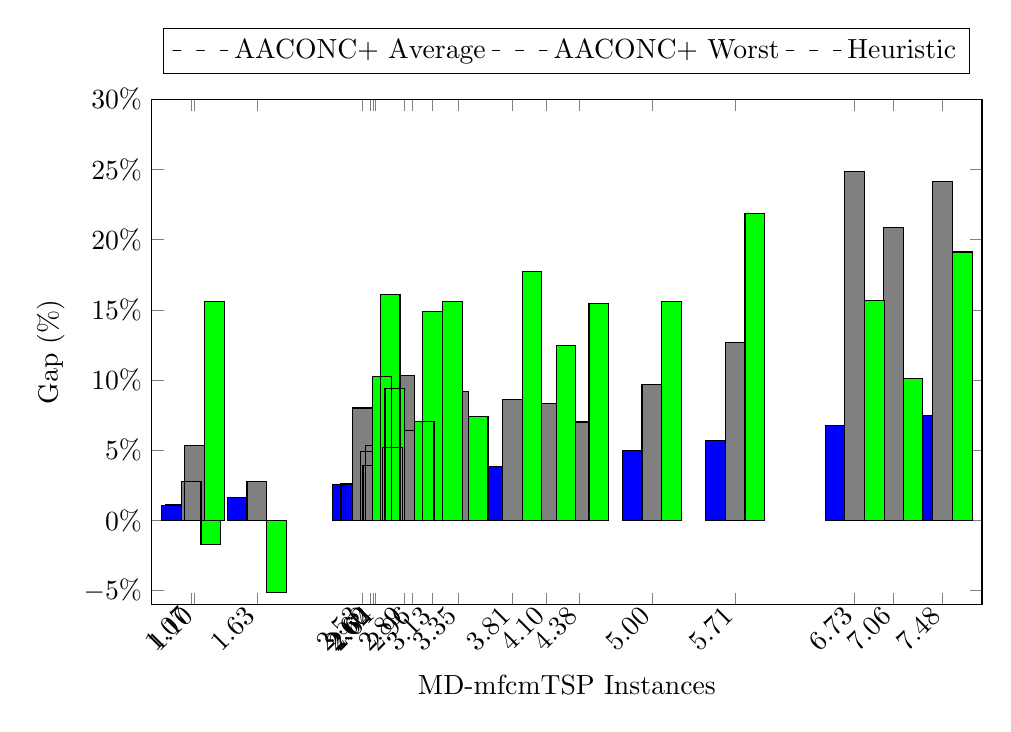
\begin{tikzpicture}
			\pgfplotstableread[col sep=comma]{
				AACOAVG, AACOWOR, HEURISTIC
				6.73, 24.88, 15.65
				7.48, 24.16, 19.12
				5.71, 12.65, 21.89
				2.89, 10.35, 7.02
				7.06, 20.84, 10.08
				2.96, 6.41, 14.86
				3.35, 9.21, 7.37
				2.53, 8.01, 10.26
				4.10, 8.32, 12.48
				2.60, 4.91, 16.08
				4.38, 7.01, 15.48
				3.81, 8.62, 17.71
				1.10, 5.31, 15.62
				3.13, 5.33, 15.57
				2.64, 5.36, 9.40
				5.00, 9.69, 15.59
				2.62, 3.93, 5.17
				1.07, 2.78, -1.69
				1.63, 2.78, -5.12
			}\datatable
			
			\begin{axis}[
				width=\textwidth,
				height=8cm,
				ymin=-6,
				ymax=30,
				ytick={-10,-5,0,5,10,15,20,25,30},
				yticklabel={\pgfmathparse{\tick}\pgfmathprintnumber{\pgfmathresult}\%},
				xtick=data,
				xticklabels from table={\datatable}{AACOAVG},
				xticklabel style={rotate=45, anchor=east},
				bar width=0.25cm,
				enlarge x limits={abs=0.5cm},
				legend style={at={(0.5,1.05)},anchor=south},
				legend columns=-1,
				ylabel={Gap (\%)},
				xlabel={MD-mfcmTSP Instances},
				title={Table 3},
				]
				
				\addplot[ybar, bar shift=-0.25cm, fill=blue] table [y=AACOAVG] {\datatable};
				\addplot[ybar, bar shift=0cm, fill=gray] table [y=AACOWOR] {\datatable};
				\addplot[ybar, bar shift=0.25cm, fill=green] table [y=HEURISTIC] {\datatable};
				
				\legend{AACONC+ Average, AACONC+ Worst, Heuristic}
			\end{axis}
		\end{tikzpicture}
		\caption{Bar plot generated using pgfplots in LaTeX.}
		\label{fig:my_bar_plot}
	\end{figure*}
